\subsubsection{UC8.1 - Personalizzazione Scatter Plot Matrix}
\begin{figure}[h]
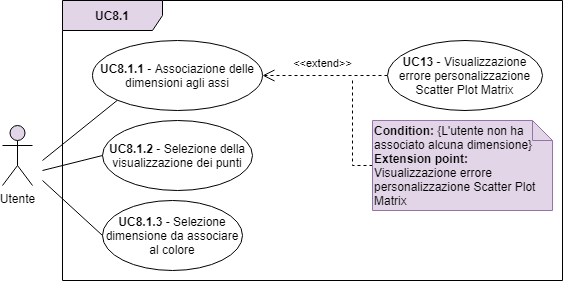
\includegraphics[width=\linewidth]{Section/Images/UC8.1.png}
\centering
\caption{UC8.1 - Personalizzazione Scatter Plot Matrix}
\end{figure}
\begin{itemize}
	\item \textbf{Attore primario}: Utente;
	
	\item \textbf{Precondizioni}: L'utente ha scelto il grafico \textit{Scatter Plot Matrix} [UC6.1];
	
	\item \textbf{Postcondizioni}: Il grafico viene aggiornato con le personalizzazioni impostate dall'utente;
	
	\item \textbf{Scenario principale}: L'utente decide:

\begin{enumerate}
\item Quali dimensioni associare ad ogni asse [UC8.1.1];
\item La forma dei punti nel grafico [UC8.1.2];
\item Quale dimensione associare al colore dei punti [UC8.1.3].
\end{enumerate}	
	
		
\end{itemize}


